\section{Optimizing for Energy and Bandwidth Usage}
\label{sec-lance}
\label{sec-utilitylance}

After completing our 2007 deployment at Tungurahua we rearchitected
our original Lance system and shifted its focus. Instead of optimizing for
storage and bandwidth, we instead chose to optimize primarily for energy,
with bandwidth as a secondary concern. Several changes to the hardware and
software environment explain this shift in emphasis.

First, storage management began to seem less pressing as the promise of
sensor network nodes with large attached flash memories seemed to be becoming
a reality.  The TMote Sky deployed at Reventador had only 1~Mbit of flash,
meaning we could only store around 20~min of signal (from two channels,
24~bits per sample at 100~Hz). In contrast, the SHIMMER mote developed for
medical monitoring can be fitted with a flash card allowing it to store as
much as 2~GB of data, meaning that deployed in support of the volcano
application it could conceivable store over 41~\textit{days} of
full-resolution sampled data (assuming 2 data channels sampled at 100~Hz with
3~bytes per sample).  The idea behind managing storage was that it was
necessary in order to preserve the highest-utility ADUs until the network
controller would get around to downloading them. Once storage sizes swelled
it seemed like a simple FIFO storage policy would allow plenty of time for
interesting data to be downloaded.

Second, support for radio duty cycling entered the TinyOS tree and began to
be used by our group. This shifted our focus from thinking about bandwidth as
a constraint to thinking about the \textit{energy} associated with operating
the radio in order to download data as a constraint. In contrast to the early
Lance system, which deployed a ``greedy'' download manager which strove to
download as much data from the network as possible, once the radio could be
easily disabled when not in use it became natural to want to consider the
cost of downloading signals and not necessarily run the downloads in a greedy
fashion. 

\subsection{Refocusing on Energy Usage}

Shifting the system's concern to energy usage required several changes to the
Lance architecture: a move from ordinal to cardinal utilities, and the
development of a cost model.

Replacing the ordinal utilities with cardinal ones allowed us to compare the
relative value of different ``baskets'' of ADUs in a meaningful way. Two
ADUs, each with a utility of 50 were considered equivalent to the application
as a single one with utility 100.  This meant that instead of simply
downloading the highest-utility ADU available in the network at a given
moment, we needed a way of determining which was the best ADU in terms of
both the value but also the system's ability to extract it.

Given our high data rates, we were already restricted by bandwidth alone to
downloading only a portion of all of the data sampled by every node in the
network.  Once we began using LPL to duty cycle the radio extracting data
also had an impact on energy consumption as well, and so achieving a given
target lifetime could be accomplished by downloading data at slower rates
allowing node radios to be powered off when not in use.  Either bandwidth or
energy could have driven the cost model, but given the dependence of energy
consumption on bandwidth usage (and lack of a similar relationship in the
other direction) we chose to represent the cost necessary to download an ADU
as the \textit{energy} required to retrieve it.

Compared with our original ordinal utility efforts, the new version of Lance
contributed several ideas. First was a way of estimating, a priori,
the energy necessary to extract an ADU from the network. This was necessary
so that both the cost and value of each ADU could be considered before
download decisions were made. For value, we leverage the same two-part
utility-assignment framework described earlier.  The cost estimation
component is described below.

In addition, once the cost and value had been assigned to each ADU, the
problem of deciding which to download can be framed as an optimization
problem. We described a way of producing an optimality bound by mapping an
offline version of this problem to a well-studied optimization problem, and
use this optimality bound to evaluate several online algorithms suitable for
real-time decision making. These contributions are also described in further
detail below.

\subsection{Cost Estimation}
\label{subsec-costassignment}

Each ADU has an associated cost $\bar{c}_i$ that represents the energy
requirement to download the ADU from the network.  $\bar{c}_i$ is a vector
$\{ c_i^1, c_i^2, \ldots, c_i^n \}$ where $c_i^j$ represents the estimated
energy expenditure of node $j$ when ADU $i$ is retrieved. The key idea is
that we explicitly model both the energy cost for downloading the ADU from
its ``host'' node $n_i$ and the energy cost for each node along the
routing path from $n_i$ to the base station which must forward packets during
the transfer. In addition, we also model the energy cost to nodes that
overhear transmissions by nodes participating in the transfer.  This energy
cost on intermediate nodes is non-negligible, since reliable transfer
protocols involve a potentially large number of retransmission. However, the
overhearing cost is typically small, since modern low-power MAC protocols
quickly return to sleep when overhearing transmissions to another node.  The
cost vector $\bar{c}_i$ therefore depends on the network topology.

Lance estimates the download energy cost vector $\bar{c}_i$ for each ADU
sampled by the network.  We assume that nodes are organized into a spanning
tree topology rooted at the base station. The cost is a function of many
factors, including the reliable transport protocol, each node's position in
the routing tree, radio link quality characteristics, and the MAC protocol. 

Given the complex dynamics that can arise during a sensor network's
operation, we opt to use a simple conservative estimate of the energy cost to
download an ADU from a node. Our approach is based on an empirical model that
captures three primitive energy costs involved in downloading an ADU. The
first, $E_d$, represents the energy used to download an ADU from a given node
which includes the energy cost for reading data from flash and sending
multiple radio packets (including any retransmissions) to the next hop in the
routing tree.  The second, $E_r$, represents the energy cost at intermediate
nodes to forward messages during the ADU transfer. The third, $E_o$,
represents the energy cost to nodes that overhear transmissions during a
transfer.  For simplicity, we assume ADUs of fixed size and compute $E_d$,
$E_r$, and $E_o$ based on the time necessary to download an ADU from the
target node.

Using this simple model, we set the elements of the cost vector $\bar{c}_i$ 
as follows. $c_i^n = E_d$ for the node $n$ hosting the ADU, and 
$c_i^m = E_r$ for nodes $m$ along the routing path from
$n$ to the base station. We set $c_i^o = E_o$ for nodes that are
assumed to be within one radio hop of any of the nodes involved in
the transfer. Estimating $\bar{c}_i$ therefore requires
knowledge of the current routing topology. This information 
is readily available: the periodic summary messages, sent to the 
base station by every node, include the node's radio neighbors and 
parent in the routing tree. Cost vectors can be easily recomputed 
whenever the routing topology changes.

To ensure that all nodes meet the lifetime target $L$, Lance models the
energy availability at each node using a token bucket with depth $D$ and fill
rate $C/L$, corresponding to the mean discharge rate.  $D$ is determined by
the target lifetime $L$, the battery capacity $B$ and the background drain
rate $R$.  In general, $D = B - L*R$, so $D$ represents the energy remaining
after the node reserves enough to ensure it can meet its target lifetime at
the background level.

\subsection{Lance Optimizer}
\label{subsec-lanceoptimizer}

The Lance optimizer is responsible for scheduling ADUs for download, based on
knowledge of the set of ADUs currently stored by the network, their
associated values, and costs.  In our design, Lance attempts to download a
single ADU at a time, in order to prevent network congestion, although it may
be possible to download multiple ADUs simultaneously, depending on the
network topology. A download completes either when the entire ADU has been
received or a timeout occurs.

Lance's optimization process attempts to maximize the value of the ADUs
retrieved while adhering to the lifetime target $L$. In essence, we seek a
greedy heuristic approximation of the multidimensional knapsack solution that
would be used by an oracle with complete knowledge of the ADUs sampled by the
network over all time.  The optimizer first excludes ADUs that would involve
nodes without enough energy to perform a download.  That is, if the token
bucket for a given node $m$ has $E(m)$ joules, ADUs for which $E(m) < c_i^m$
are excluded from consideration.  Note that as the bucket fills, the ADU may
become available for download at a later time. We call these ADUs {\em
infeasible}, and the remaining {\em feasible}.

To determine the next ADU to download, the optimizer considers the 
value $v_i$ of each ADU and the its associated cost $\bar{c}_i$.
We consider three {\em scoring functions} that assign a 
download score to each feasible ADU; the ADU with the highest download score
is downloaded next. In the case of ties, an arbitrary ADU is chosen.

The first scoring function, {\em value-only}, simply downloads the feasible
ADU with the highest value $v_i$. Note that {\em value-only} will meet the
network's lifetime target (since only feasible ADUs are considered) but does
not rank ADUs according to cost.  The second scoring function, {\em
cost-total}, assigns the score $\hat{v}_i$ by scaling the value of the ADU by
its total cost: $\hat{v}_i = v_i / \sum_j c_i^j$. The feasible ADU with the
highest score is then downloaded from the network. This approach penalizes
ADUs stored deep in the routing tree, which have a higher overall cost than
those located near the base station. 

The third scoring function, {\em cost-bottleneck}, scales the ADU value $v_i$
by the cost to the node that is an energy bottleneck for downloading this
ADU. That is, let $b$ represent the node with the minimum value of $E(b)$
such that $c_i^b > 0$. {\em cost-bottleneck} sets the score $\hat{v}_i = v_i
/ c_i^b$. The intuition behind this scoring function is that the most
energy-constrained node should be considered when scoring ADUs for download.
We evaluate all three scoring functions in the next section and show that
they yield very different results in terms of spatial distribution and energy
efficiency.

We evaluate each scoring function against an optimal solution calculated by
using knowledge of all future ADUs and solving the multi-dimensional knapsack
problem. Since an online solution is required, this provides an upper bound on
the achievable performance of the online scoring functions.

\subsection{Evaluation and Results}
\label{subsec-evaluationandresults}

Prior work~\cite{lance-sensys08} presents a thorough and detailed evaluation
of Lance on a variety of real and synthetic workloads, evaluated both in
simulation and in experiments on a large sensor network
testbed~\cite{motelab}.  We present a subset of these results here to further
the discussion.

\subsubsection{Simulation and Testbed Experiments}

We began by evaluating Lance using a realistic system simulator which allowed
parameters -- ADU size, distribution of ADU values, network topologies,
download speeds, energy costs and target lifetimes to be easily varied. Our
simulations focus first on evaluating the candidate scoring functions described
above, and secondly on assessing the performance of Lance as the parameters
above are varied.

\begin{figure}[t]
\begin{center}
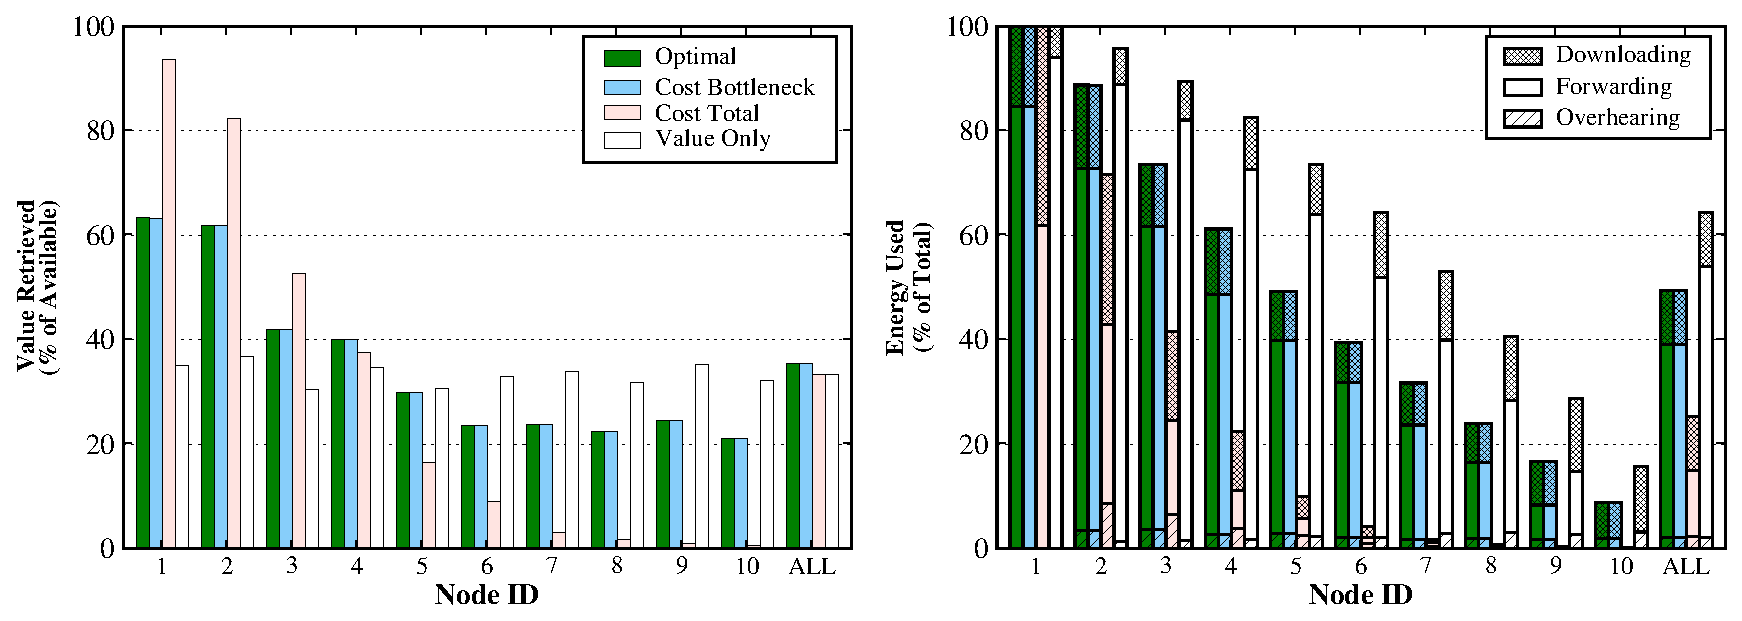
\includegraphics[width=1.0\hsize]{./figs/Sensys2008/2008-lance-linearsimulation.eps}
\end{center}
\caption{{\bf Per-node distribution of ADU value and energy usage for the
linear simulation experiment.} 
The left graph shows the amount of data value downloaded from each node,
while the right graph breaks down the amount of energy used by each node into
the downloading, routing and overhearing components. Node~1 is closest to
the base station.}
\label{fig-lance-linearsimulation}
\end{figure}

Our first simulation experiment used a simple 10-node linear topology.
Figure~\ref{fig-lance-linearsimulation} shows both the performance of each
scoring function against the offline optimal system and a breakdown of the
estimated energy consumed on each node during the simulation. We divide each
node's energy usage into three components: \textit{downloading} energy
consumed by the node when it is transferring one of its own ADUs to the base
station, \textit{forwarding} energy consumed while transferring data upstream
for a downstream node, and \textit{overhearing} energy which accounts for the
small overhearing penalty imposed by the TinyOS LPL implementation on nodes
that overhear (but are not participating in) nearby transfers.

The energy costs for various operations are modeled as follows.  The
background current drain of each node is set to 2~mA, based on empirical
measurements of a TMote~Sky sensor node performing high-data-rate sampling and
storing to flash.  We also measured the current consumption to download an ADU
from a sensor node, and derived the energy costs for downloading ($E_d =
17.6$~mA), routing ($E_r = 16.9$~mA), and overhearing ($E_o = 2$~mA).
Our experiments assume that each node can only overhear its parent in the
routing tree; developing more detailed overhearing models is the subject of
future work.  Computing the components of the cost vector for a particular ADU
is done by multiplying the current consumption by the ADU download time for
each node either downloading, routing, or overhearing the transmission.

Figure~\ref{fig-lance-linearsimulation} confirms the intuition behind the
scoring function behavior.  \emph{value-only} downloads roughly equal value
from each node, but fails to match the optimal performance. \emph{cost-total}
downloads more data from nodes near the sink.  \emph{cost-bottleneck} comes
close to matching the optimal solution, retrieving over 99\% of the value
retrieved by the optimal solution.

\begin{figure}[t]
\caption{{\bf Optimality of different scoring functions.} 
This table summarizes simulation results evaluating the three different
scoring functions.  Results are shown for several different lifetime targets
and value distributions.  {\em cost-bottleneck} out-performs the others in
almost all cases.}
\vspace{0.2in}
\begin{center}
\begin{tabular}{llccc}
\noalign{\smallskip}
& & \multicolumn{3}{c}{Scoring Functions} \\
& & Value & Cost & Cost \\
Distribution & Lifetime & Only & Total & Bottleneck \\
\noalign{\smallskip}\svhline\noalign{\smallskip}
\multirow{3}{*}{Uniform} & 4 months & 62.4\% & 90.5\% & \textbf{93.2\%} \\
& 11 months & 43.4\% & 68.0\% & \textbf{96.9\%} \\
& 18 months & 44.6\% & 49.0\% & \textbf{90.0\%} \\
\noalign{\smallskip}\svhline\noalign{\smallskip}
\multirow{3}{*}{Exponential} & 4 months & 83.9\% & 85.1\% & \textbf{88.0\%}
\\
& 11 months & 70.4\% & 82.0\% & \textbf{93.0\%} \\
& 18 months & 67.2\% & 72.8\% & \textbf{91.2\%} \\
\noalign{\smallskip}\svhline\noalign{\smallskip}
\multirow{3}{*}{Zipfian} & 4 months & 84.7\% & \textbf{91.4\%} & 87.1\% \\
& 11 months & 63.8\% & 91.1\% & \textbf{96.2\%} \\
& 18 months & 53.1\% & 86.9\% & \textbf{93.8\%} \\
\end{tabular}
\end{center}
\label{fig-lancetable}
\end{figure}

To confirm our intuition we ran a set of simulations using a more realistic
25-node tree topology and using a variety of different ADU value
distributions.  We draw ADU values from several distributions in an attempt to
understand Lance's behavior as the properties of the sampled data change.
Three value distributions are used: uniform random, exponentially distributed,
and Zipf with exponent $\alpha = 1$.  We also make use of an ADU value
distribution based on a 6~hour seismic signal collected at Reventador Volcano,
Ecuador in 2005~\cite{volcano-osdi06} for a later experiment.
Table~\ref{fig-lancetable} summarizes the results, showing that the {\em
cost-bottleneck} scoring function outperforms the other two in most cases,
with optimality values between 87.1\% and 96.9\%.  The one exception is the
4-month Zipfian data set, where \emph{cost-total} slightly outperforms
\emph{cost-bottleneck}.

\begin{figure}[t]
\begin{center}
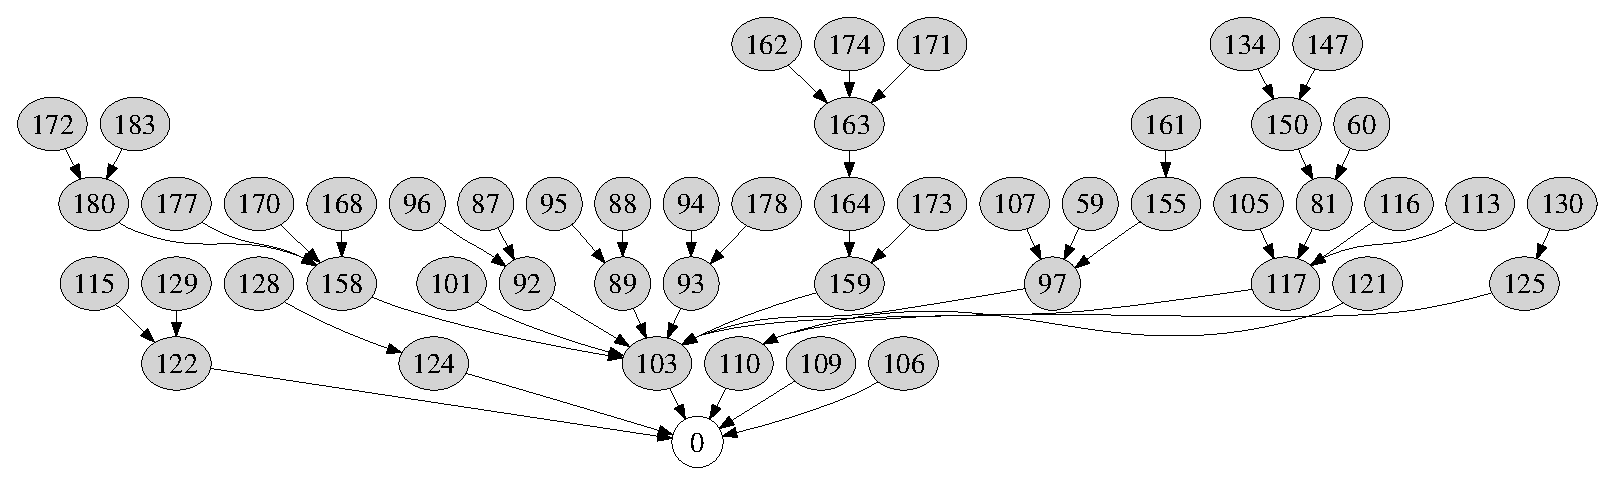
\includegraphics[width=1.0\hsize]{./figs/Sensys2008/2008-lance-testbed-topology.eps}
\end{center}
\caption{{\bf Topology for testbed experiments.} 
This graph shows the 50 node topology used for the testbed experiments shown
in Fig.~\ref{fig-lance-testbed}.}
\label{fig-lance-testbed-topology}
\end{figure}

\begin{figure}[t]
\begin{center}
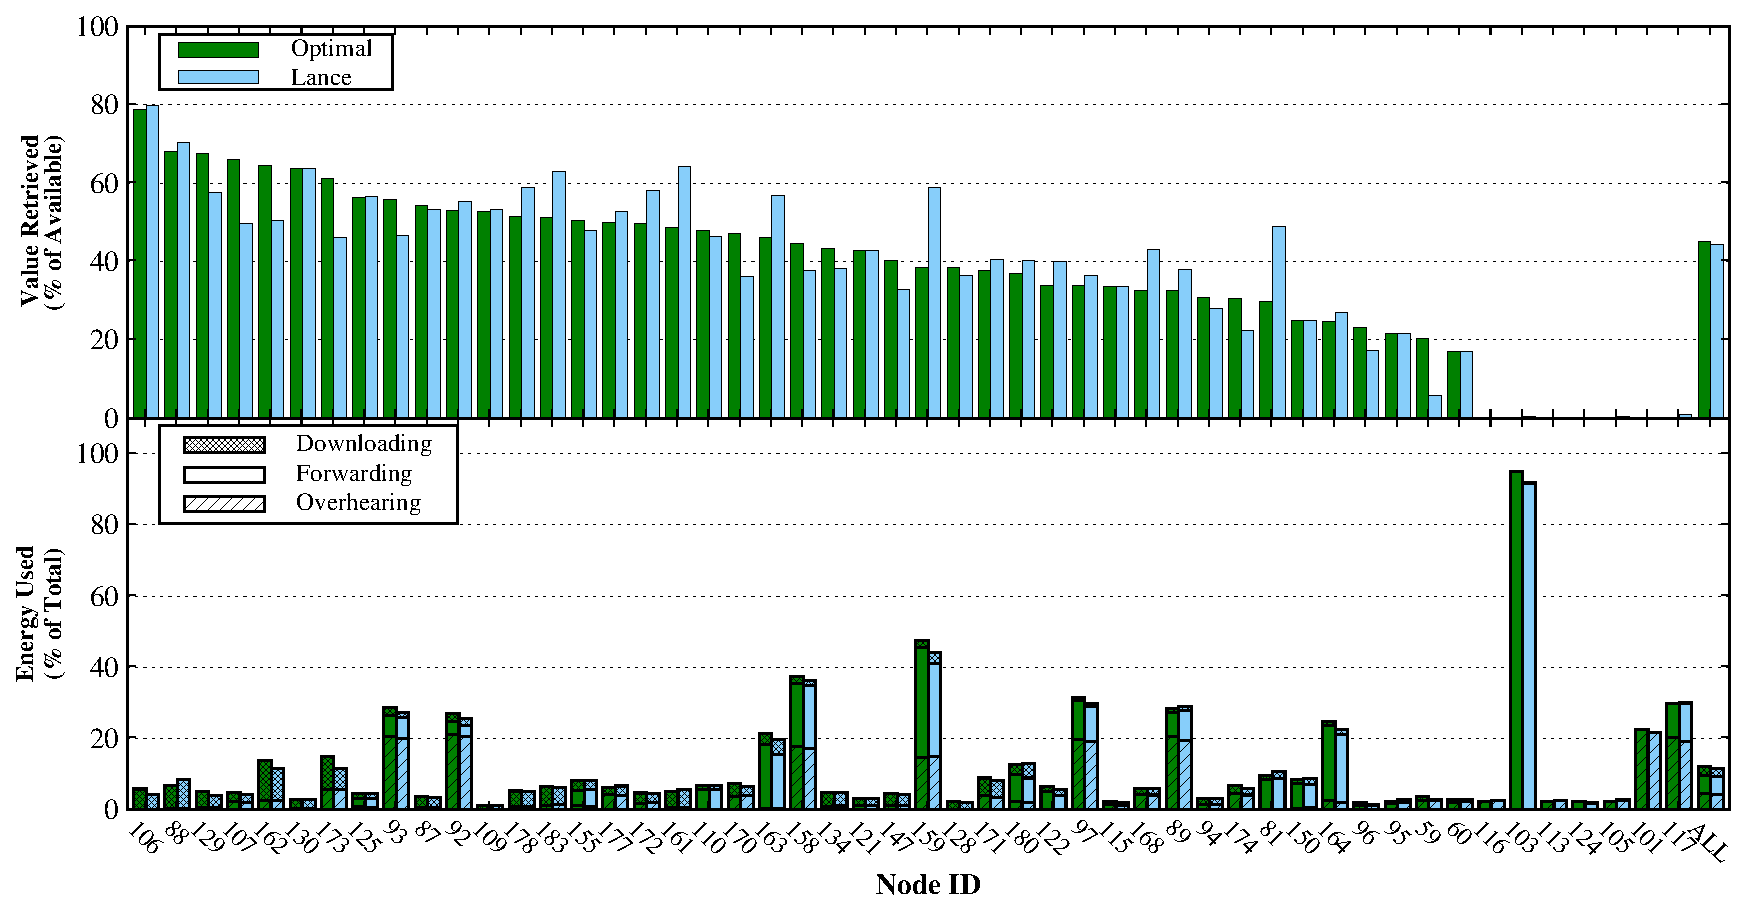
\includegraphics[width=1.0\hsize]{./figs/Sensys2008/2008-lance-testbed.eps}
\end{center}
\caption{{\bf Optimality and energy use in the 50-node testbed experiment.}
Lance achieved near-optimal performance during this 8-hour testbed
experiment, retrieving 98\% of the value obtained by the offline optimal
algorithm.}
\label{fig-lance-testbed}
\end{figure}

We also ran Lance on our MoteLab~\cite{motelab} Wireless Sensor Network
Testbed, in a 50-node configurations shown in
Fig.~\ref{fig-lance-testbed-topology}. These experiments stress the system in a
realistic setting subject to radio interference and congestion, and exercise
the multihop routing protocol, Fetch reliable data-collection protocol, and
ADU summary traffic generated by the nodes. For these experiments, we
injected artificial ADU values directly into each node rather than relying on
the nodes sampling real sensor data; this approach allows us to perform
repeatable experiments that explore a wider range of ADU value distributions.
We use the \emph{cost-bottleneck} scoring function. 

Figure~\ref{fig-lance-testbed} shows the results of a 50-node testbed
experiment using a Zipfian data distribution and a target lifetime of
6~months.  The upper portion of the figure shows the amount of data value
obtained by Lance from each node, compared to the optimal solution (which was
computed offline). Nodes are sorted by decreasing optimal value. As the
figure shows, Lance achieves very close to the optimal solution, with an
optimality of 98\% overall.  In some cases, Lance incorrectly downloads more
data from some nodes and less data from others; this is due to the inherent
limitations of an online solution that cannot foresee future ADU values.  The
lower portion of the figure shows the energy breakdown for each node with
downloading, forwarding, and overhearing costs shown.  Some nodes consume
more than others because of their location in the routing tree. For example,
node~103 in uses a great deal of energy for routing packets as it is one hop
from the base station, although no ADUs are ever downloaded from that node.

\subsubsection{2007 Deployment Analysis}

While the earlier, priority-based version of Lance was used to drive our 2007
deployment at Tungurahua, we were still able to analyze this system's
performance using utility-based metrics.  To evaluate Lance's behavior with
respect to an ``optimal'' system, we took the 8483~RSAM summaries received
during a 16-hour period when the debiasing filter (see
Sect.~\ref{subsec-policymoduleuse}) was enabled. Using this
information, we compute the set of ADUs that the optimal system would have
downloaded, with complete knowledge of all ADUs but limited to the same time
duration the original network was operating.  We assume the download
throughput for a given node is always the mean throughput for that node
observed during the deployment (see Fig.~\ref{fig-throughputtable}). This
calculation ignores energy constraints because the deployed system did not
consider energy costs.

An optimal system would have downloaded 392~out of the~8483 ADUs,
whereas the actual system downloaded 418~ADUs during this 
time.\footnote{The optimal system would download fewer ADUs 
than the real system due to the variation in the throughput to each 
node: the optimal system would download more ADUs from nodes 
with lower throughput, thereby limiting the total number of ADUs it could
download.} The total value of ADUs downloaded by the optimal system 
is 10678, whereas the value of the actual network was 10629, for an
optimality of 99.5\%. Lance did an exceptional job of extracting the
highest-value data from the network using our online heuristic
algorithm.

We can perform a similar analysis during the period of time during which the
network was using the EWMA-based summarization function. As with the
RSAM-based summarization function, we estimate the optimal set of ADUs that an
oracle would have downloaded. During a 25-hour period, the network reported
11012~unique ADU summaries. An optimal system would have downloaded 554 ADUs
with total value 577377.  The actual network downloaded 518~ADUs with a value
of 539115, for an optimality of 93.3\%. 

As a final evaluation metric, we wish to consider how well Lance, configured
in this manner, was able to download seismic signals representing earthquakes.
Given the low level of volcanic activity, it turns out that most of the ADUs
downloaded by Lance contain no discernible seismic signal. In fact, upon
manual inspection of the 518~ADUs downloaded during this period, we identified
only 20~ADUs showing a clear earthquake signal, corresponding to only
9~separate seismic events.  Note that we did {\em not} configure Lance to
explicitly download correlated earthquakes by using an appropriate policy
module (described in Sect.~\ref{sec-policymodules}), so we would not expect
a high degree of coverage for the same event across multiple nodes.

\begin{figure}[t]
\begin{center}
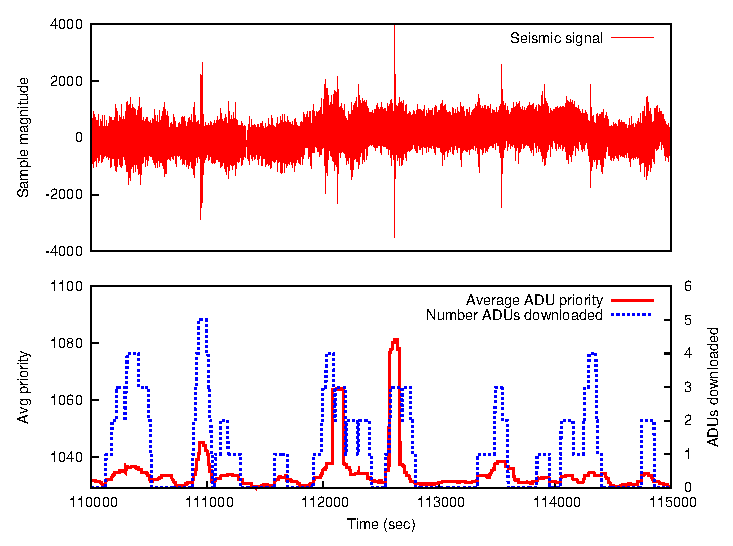
\includegraphics[width=1.0\hsize]{./figs/Sensys2008/2008-lance-download-behavior.eps}
\end{center}
\caption{{\bf Lance download behavior overlaid with average ADU value.}
The top plot shows the continuous seismic signal collected by a single node.
The lower plot shows the average value of ADUs and the number of ADUs
downloaded for each window.}
\label{fig-lance-download-behavior}
\end{figure}

Figure~\ref{fig-lance-download-behavior} shows the behavior of Lance during a
representative 83-minute period. In the figure, we have broken time into
windows of one-half an ADU duration (55~sec in this case), and computed the
mean ADU value as well as the number of downloaded ADUs that overlap each time
window. As the data shows, elevated seismic activity is well-correlated with
an increase in the ADU value from across the network, as well as the number of
downloaded ADUs.  Moreover, the few cases of clear seismic activity in the
trace (at times 111000, 112700, and so forth) tend to have more ADUs
downloaded. Of the 9~separate seismic events, a total of 27~ADUs were
downloaded, representing a per-event ``coverage'' of 3~ADUs per event.  This
represents just under half of the 7~nodes participating in the network.


\subsubsection{Results Summary}

To summarize the results, we found that the cost
bottleneck scoring function allows Lance to approach optimal performance
across a variety of network sizes, bandwidth distributions and target
lifetimes.  By directing scarce energy resources towards the most valuable
data, the overall efficiency of the network considered as a whole can be
significantly increased.
